\documentclass[11pt,a4paper,openany]{article}
\usepackage{lscape,overcite,chapterbib}
\usepackage{longtable}
\usepackage{supertabular}
\usepackage{color}
\usepackage[dvipdfmx]{graphicx}


\usepackage{ascmac}
\usepackage{amsmath,amsthm,amssymb}
\usepackage{cancel}
\usepackage{bm}

\allowdisplaybreaks[1]

\usepackage{indentfirst}
%\usepackage[mathscr]{eucal}
\usepackage{mathrsfs}
\usepackage{upgreek}

%\renewcommand{\baselinestretch}{1.5}

\setlength{\oddsidemargin}{-1mm}
\setlength{\evensidemargin}{-4mm}
\setlength{\topmargin}{-10mm}
\setlength{\textwidth}{160mm}
\setlength{\textheight}{247mm}

\begin{document}

%----- title -----
\pagestyle{empty}
{\textbf{}}
\vspace{30mm}
\begin{center}
{\bf
\Huge{d77 User Manual} \\
\vspace{10mm} 
\vspace{100mm}       
\LARGE{Shizu Katsuyuki (志津 功將)}\\
\vspace{10mm} 
\LARGE{2024}
}
\end{center}
\clearpage
%---------------

\pagestyle{plain}
\pagenumbering{arabic}

%\section{Preface}
%d77 is a FORTRAN code for visually understanding molecular properties.

\section{License}
\noindent
d77 is free software and can be redistributed and/or modified
under the terms of the GNU General Public License v3.0
as published by the Free Software Foundation.
For details, see https://www.gnu.org/licenses/gpl-3.0.html.

\section{Citation}
\noindent
You can cite d77 as\vspace{3mm}\\
d77: visual understanding of molecular properties. Version 20240427. https://github.com/\\
KatsuyukiShizu/d77\\

\noindent
BibTex description:
\begin{verbatim}
@misc{d77,
title = {
d77: visual understanding of molecular properties. 
Version 20240427. https://github.com/KatsuyukiShizu/d77
}
}
\end{verbatim}

\section{Notations}
\noindent
\begin{tabular}{ll}
PGF & primitive Gaussian function\\
CGF & contracted Gaussian function\\
VCC & vibronic coupling constant\\
SOC & spin-orbit coupling\\
fchk file & formatted checkpoint file\\
TD-DFT & time-dependent density functional theory\\
CI & configuration interaction\\
CIS & configuration interaction singles\\
$\rho_{n}$ & electron density of electronic state $| n \rangle$\\
$\rho_{mn}$ & overlap (transition) density between electronic states $| m \rangle$ and $| n \rangle$\\
$\Delta\rho_{mn}$ & electron-density difference: $\rho_{m}-\rho_{n}$\\
$\bm{\upmu}$ & permanent/transition dipole moment \\
$\tau_x$ & permanent/transition dipole moment density in the $x$ direction\\
$\tau_y$ & permanent/transition dipole moment density in the $y$ direction\\
$\tau_z$ & permanent/transition dipole moment density in the $z$ direction\\
$\tau_{\bm{\upmu}}$ & permanent/transition dipole moment density in the direction of $\bm{\upmu}$\\
$\nu_k$ & derivative of the nuclear electronic potential for the $k$th vibrational mode\\
$\eta_k$ & vibronic coupling density for the $k$th vibrational mode
\end{tabular}
%%%%%%%%%%%%%%%%%%%%%%%%%%%%%%%%%%%%%%%%%%%%%%%%%%%%%%%%%%%%%%%%%%%%%%%%%%%%%%%%%%%%%%%%%%%%
%%%%%%%%%%%%%%%%%%%%%%%%%%%%%%%%%%%%%%%%%%%%%%%%%%%%%%%%%%%%%%%%%%%%%%%%%%%%%%%%%%%%%%%%%%%%
\clearpage
\section{Compiling and running  d77}
\noindent
You can download Fortran90 source files, documents, and examples from 
GitHub:\cite{d77}\\
https://github.com/KatsuyukiShizu/d77\\
Shell scripts (d77.sh and run\_d77.sh), Fortran90 source files, and Makefile are in the src directory.
Go to your src directory and type:
\begin{verbatim}
make
\end{verbatim}
The executable file (d77.exe) is created in your src directory.\\

The default settings for 
the maximum number of electrons (Max\_ne),
the maximum number of atoms (Max\_n\_atm), 
the maximum number of vibrational modes (Max\_n\_mode),
the maximum number of CGFs (Max\_n\_cgf),
the maximum number of PGFs for each CGF (Max\_n\_pgf), 
and
the maximum number of electronic configurations (Max\_n\_elec\_config) 
are defined in a module, global\_constants.f90:
\begin{verbatim}
Max_ne = 100
Max_n_atm = 30
Max_n_mode = 100
Max_n_cgf = 1000
Max_n_pgf = 30
Max_n_state = 20
Max_n_elec_config = 1000
\end{verbatim}
Change the default settings depending on your computer's system environment.\\

Utility programs for d77 are in the src/util directory. 
A utility program, dpp, performs data preprocessing for d77.
dpp extracts data from Gaussian 16 output files (fchk and log files) and
saves them to INP\_ELEC and/or INP\_VIB directory. 
Shell scripts (dpp.sh and others) are in the src/util/dpp directory. 
Fortran90 source files and Makefile are in the src/util/dpp/f90 directory. 
Go to your src/util/dpp/f90 directory and type:
\begin{verbatim}
make
\end{verbatim}
The executable file (dpp.exe) is created in your src/util/dpp/f90 directory.\\

Edit your configuration file, for example, .bashrc:
\begin{verbatim} 
alias d77='sh ABCD/d77/src/d77.sh'
export DIR_d77_EXE=ABCD/d77/src
alias dpp='sh ABCD/d77/src/util/dpp/dpp.sh'
export DIR_d77_dpp_f90=ABCD/d77/src/util/dpp/f90
\end{verbatim} 
Here, ABCD is a directory where you created d77 directory.
To run d77, simply type:
\begin{verbatim} 
d77 'input file' 'results directory'
\end{verbatim}
If you have an input file, \textit{test.inp}, and want to save the log file (\textit{test.log}) and calculated data to \textit{res\_test} directory, type:
\begin{verbatim} 
d77 test.inp res_test
\end{verbatim}
or 
\begin{verbatim} 
d77 test res_test
\end{verbatim}
You can run the job without specifying a results directory:
\begin{verbatim} 
d77 test
\end{verbatim}
In this case, the log file and calculated data are saved to \textit{test} directory.

%%%%%%%%%%%%%%%%%%%%%%%%%%%%%%%%%%%%%%%%%%%%%%%%%%%%%%%%%%%%%%%%%%%%%%%%%%%%%%%%%%%%%%%%%%%%
%%%%%%%%%%%%%%%%%%%%%%%%%%%%%%%%%%%%%%%%%%%%%%%%%%%%%%%%%%%%%%%%%%%%%%%%%%%%%%%%%%%%%%%%%%%%
\clearpage
\section{Input file description}

\subsection{Comment lines}
\noindent
Add comments between \$comment and \$end\_comment lines in your input file. Comment lines have no influence on d77 execution.

\subsection{Control options}
\noindent
Add control options between \$control and \$end\_control lines.

\begin{verbatim}
property
\end{verbatim}
\begin{tabular}{ll}
dipole & calculates permanent/transition dipole moment (default).\\
vc & calculates diagonal/off-diagonal VCC. \\
soc & calculates SOC between singlet and triplet states.\\
rho & calculates electron density or overlap (transition) density if runtyp = density.
\end{tabular}
\\

\begin{verbatim}
runtyp
\end{verbatim}
\begin{tabular}{ll}
calc\_int\_cgf & calculates one-electron integrals between CGFs\\
                   & with the McMurchie and Davidson formulation.\cite{MCMURCHIE1978218} \\
int\_pgf & calculates molecular properties from one-electron integrals between PGFs \\
           & with the McMurchie and Davidson formulation\cite{MCMURCHIE1978218}  (default).\\
density & calculates molecular property densities and writes them to cube files.\\
cube & manipulates existing cube files and generates a new cube file.\\
\end{tabular}
\\

\begin{verbatim}
method
\end{verbatim}
\begin{tabular}{ll}
td & reads $\bf{X}$ and $\bf{Y}$ calculated with TD-DFT (default). \\
cis & reads CI coefficients calculated with CIS. 
\end{tabular}
\\

\begin{verbatim}
effcharg_soc
\end{verbatim}
\begin{tabular}{ll}
read & reads effective nuclear charges from ZEFF\_SOC file (default). \\
koseki & uses Koseki's effective nuclear charges.\cite{doi:10.1021/j100205a033, doi:10.1021/j100034a013, doi:10.1021/jp983453n} \\
nuccharg & uses nuclear charges as effective nuclear charges for SOC calculation.
\end{tabular}
\\

\begin{verbatim}
cube_op
\end{verbatim}
\begin{tabular}{ll}
add & adds two cube files and saves the calculated date to a new cube file.\\
sub & subtracts two cube files and saves the calculated date to a new cube file.\\
mul & multiplies two cube files and saves the calculated date to a new cube file.\\
\end{tabular}

\subsection{Spin-orbit coupling options}
\noindent
Add spin-orbit coupling options between \$spin\_orbit and \$end\_spin\_orbit lines.
\begin{verbatim}
ms
\end{verbatim}
\begin{tabular}{rl}
$0$ & calculates SOC between singlet and triplet states with $M_{\rm{s}} = 0$ (default).\\
$1$ & calculates SOC between singlet and triplet states with $M_{\rm{s}} = 1$.\\
$-1$ & calculates SOC between singlet and triplet states with $M_{\rm{s}} = -1$.
\end{tabular}
\\

\subsection{Electronic state options}
\noindent
Add electronic state options between \$elec\_state and \$end\_elec\_state lines.
\begin{verbatim}
bra
\end{verbatim}
\begin{tabular}{ll}
$\langle 0 |$ & ground state (default)\\
$\langle n |$ & $n$th excited state ($n \geq 1$)
\end{tabular}
\begin{verbatim}
ket
\end{verbatim}
\begin{tabular}{ll}
$| 0 \rangle$ & ground state (default)\\
$| n \rangle$ & $n$th excited state ($n \geq 1$)
\end{tabular}
\\
\vspace{5mm} 
\\
The following description calculates molecular properties between the first and third excited states:
\begin{verbatim}
$elec_state
bra = < 1 |
ket = | 3 >
$end_elec_state
\end{verbatim}

\subsection{Grid options}
\noindent
Grid options are valid if runtyp = density.
Add the grid options between \$grid and \$end\_grid lines.\\

\begin{tabular}{ll}
xmin & minimum $x$ coordinate in bohr\\
xmax & maximum $x$ coordinate in bohr\\
ymin & minimum $y$ coordinate in bohr\\
ymax & maximum $y$ coordinate in bohr\\
zmin & minimum $z$ coordinate in bohr\\
zmax & maximum $z$ coordinate in bohr\\
dx & grid spacing in $x$ direction (the default value is 0.25 bohr)\\
dy & grid spacing in $y$ direction (the default value is 0.25 bohr)\\
dz & grid spacing in $z$ direction (the default value is 0.25 bohr)
\end{tabular}
\\

\subsection{Input data directories}
\noindent
Add input data directories in your input file. 
If your INP\_ELEC, INP\_VIB, ELFLD, and SOC\_CGF directories are in the same directory 
where your input file is, add the following descriptions:
\begin{verbatim}
INPDIR_ELEC = INP_ELEC
INPDIR_VIB = INP_VIB
INPDIR_ELFLD = ELFLD
INPDIR_SOC_CGF = SOC_CGF
\end{verbatim}

%%%%%%%%%%%%%%%%%%%%%%%%%%%%%%%%%%%%%%%%%%%%%%%%%%%%%%%%%%%%%%%%%%%%%%%%%%%%%%%%%%%%%%%%%%%%
%%%%%%%%%%%%%%%%%%%%%%%%%%%%%%%%%%%%%%%%%%%%%%%%%%%%%%%%%%%%%%%%%%%%%%%%%%%%%%%%%%%%%%%%%%%%
\clearpage
\section{Examples}

\subsection{VCCs between singlet/triplet states at optimized S$_0$ geometry}\label{calc_VCC}
This example shows how VCCs are calculated with d77. 
Sample d77 input and output files are in the
examples/C2H4 and 
examples/C2H4/VC directories.

\begin{enumerate}
\item{
Run geometry optimization and frequency analysis with Gaussian 16.\cite{g16} 
6D and 10F options are required to run d77.
}

\begin{enumerate}
\item{
Input description for geometry optimization
\begin{verbatim}
#P B3LYP/6-31G(d)
6D 10F
opt
\end{verbatim}
}

\item{
Input description for frequency analysis 
\begin{verbatim}
%chk=freq.chk
#P B3LYP/6-31G(d)
6D 10F
Freq=HPModes
\end{verbatim}
}

\item{
Input description for excited-state calculation with TD-DFT
\begin{verbatim}
%chk=TD.chk
#P B3LYP/6-31G(d)
6D 10F
TD(50-50, Nstates=5)
IOP(9/40=4)
\end{verbatim}
}
\end{enumerate}

\item{
Generate fchk files from the checkpoint files.  
Use the formchk utility of the Gaussian 16 program:
\begin{verbatim}
formchk freq.chk
formchk TD.chk
\end{verbatim}
}
Confirm that freq.fchk and TD.fchk files are generated. 
Sample freq.fchk, TD.fchk, and TD.log files are in the examples/C2H4 directory.

\item{
Create an input file (dpp.inp) for data preprocessing and run dpp. dpp.inp is formatted as follows:
\begin{verbatim}
QC_PROGRAM_ELEC = g16
QC_PROGRAM_VIB  = g16
QC_METHOD = td
PROPERTY = vc

THRESHOLD_CICOEF = 1.0D-4

DATA_ELEC_MODELSYS = TD.fchk
DATA_CICOEF_MODELSYS = TD.log
DATA_VIB_REALSYS = freq.fchk
\end{verbatim}
To run dpp, type:
\begin{verbatim} 
dpp
\end{verbatim}
INP\_ELEC and INP\_VIB directories are created. Sample INP\_ELEC and INP\_VIB directories are in the examples/C2H4 directory.
}

\item{
Calculate electric field integrals between CGFs with d77.\\
A sample input file (ELFLD.inp) is as follows:
\begin{verbatim}
$comment
Input file for calculating electric field integrals between CGFs
$end_comment

$control
property = vc
runtyp   = calc_int_cgf
$end_control

DIR_INP_ELEC = INP_ELEC
\end{verbatim}
To run d77, type:
\begin{verbatim} 
d77 ELFLD
\end{verbatim}
d77 reads information on the nuclear coordinates and atomic orbitals from \\
INP\_ELEC directory, calculates the electric field integrals, and writes them to a file (ELFLD\_CGF\_ATM) in the ELFLD directory. 
Note that ELFLD\_CGF\_ATM takes up large amounts of disk space (sometimes larger than 10 GB) for large molecules. 
A sample ELFLD\_CGF\_ATM file is in the examples/C2H4/ELFLD directory.
}

\item{
Calculate VCCs between S$_0$ and S$_1$ from the electric field integrals.\\
Create VC directory and move into it:
\begin{verbatim}
mkdir VC
cd VC
\end{verbatim} 
A sample input file (VC\_0\_3.inp) is as follows:
\begin{verbatim} 
$comment
Input file for calculating vibronic coupling constants
between S0 and S1
| 0 > : ground state (S0)
| 3 > : lowest excited singlet state (S1)
$end_comment

$control
property = vc
runtyp   = int_pgf
method   = td
$end_control

$elec_state
bra = < 0 |
ket = | 3 >
$end_elec_state

DIR_INP_ELEC  = ../INP_ELEC
DIR_INP_VIB   = ../INP_VIB
DIR_INP_ELFLD = ../ELFLD
\end{verbatim}
To run d77, type:
\begin{verbatim} 
d77 VC_0_3
\end{verbatim}
The frequencies (in cm$^{-1}$) and calculated S$_0$-S$_1$ VCCs (in atomic units) are written in VC\_0\_3.log and VCC files in VC\_0\_3 directory. The transition dipole moments between S$_0$ and S$_1$ are also written in VC\_0\_3.log (in atomic units and debye) and DM files (in atomic units) in the VC\_0\_3 directory.}

\item{
Calculate VCCs between T$_1$ and T$_2$ from the electric field integrals.\\
A sample input file (VC\_1\_2.inp) is as follows:
\begin{verbatim} 
$comment
Input file for calculating vibronic coupling constants
between T1 and T2
| 1 > : lowest triplet state (T1)
| 2 > : second lowest triplet state (T2)
$comment

$control
property = vc
runtyp   = int_pgf
method   = td
$end_control

$elec_state
bra = < 1 |
ket = | 2 >
$end_elec_state

DIR_INP_ELEC  = ../INP_ELEC
DIR_INP_VIB   = ../INP_VIB
DIR_INP_ELFLD = ../ELFLD
\end{verbatim}
To run d77, type:
\begin{verbatim} 
d77 VC_1_2
\end{verbatim}
}
\end{enumerate}

%%%%%%%%%%%%%%%%%%%%%%%%%%%%%%%%%%%%%%%%%%%%%%%%%%%%%%%%%%%%%%%%%%%%%%%%%%%%%%%%%%%%%%%%%%%%
%%%%%%%%%%%%%%%%%%%%%%%%%%%%%%%%%%%%%%%%%%%%%%%%%%%%%%%%%%%%%%%%%%%%%%%%%%%%%%%%%%%%%%%%%%%%
\subsection{SOCs between singlet and triplet states at optimized S$_0$ geometry}
This example shows how SOCs are calculated with d77. Sample d77 input and output files are in the examples/C2H4/SOC directories. The first three steps are the same as in \bf{\ref{calc_VCC}}\rm{.}

\begin{enumerate}

\item{
Run geometry optimization and frequency analysis with Gaussian 16. 
6D and 10F options are required to run d77.
}
\item{Generate freq.fchk and TD.fchk files.}
\item{Run dpp.}

\item{
Calculate SOC integrals between CGFs with d77.\\
A sample input file (SOC\_CGF.inp) is as follows:
\begin{verbatim}
$comment
Input file for calculating spin-orbit integrals between CGFs
$end_comment

$control
property = soc
runtyp   = calc_int_cgf
$end_control

DIR_INP_ELEC = INP_ELEC
\end{verbatim}
To run d77, type:
\begin{verbatim} 
d77 SOC_CGF
\end{verbatim}
d77 reads information on the nuclear coordinates and atomic orbitals from \\
the INP\_ELEC directroy, calculates the spin-orbit integrals, 
and writes them to files (SOC\_CGF\_X, SOC\_CGF\_Y, and SOC\_CGF\_Z) in the SOC\_CGF directory.
}

\item{
Calculate $x$, $y$, and $z$ components of SOC between S$_0$ and T$_1$ 
with $M_{\rm{s}} = 0$ from the SOC integrals between CGFs.\\
Create SOC directory and move into it:
\begin{verbatim}
mkdir SOC
cd SOC
\end{verbatim} 
A sample input file (SOC\_0\_1\_Ms\_0.inp) is as follows:
\begin{verbatim} 
$comment
Input file for calculating spin-orbit coupling
between S0 and T1 (Ms = 0)
| 0 > : ground state (S0)
| 1 > : lowest triplet state (T1)
$end_comment

$control
property     = soc
runtyp       = int_pgf
method       = td
effcharg_soc = read
$end_control

$spin_orbit
ms = 0
$end_spin_orbit

$elec_state
bra = < 0 |
ket = | 1 >
$end_elec_state

DIR_INP_ELEC    = ../INP_ELEC
DIR_INP_SOC_CGF = ../SOC_CGF
\end{verbatim}
To run d77, type:
\begin{verbatim} 
d77 SOC_0_1_Ms_0
\end{verbatim}
The calculated $x$, $y$, and $z$ components of S$_0$-T$_1$ SOC are written 
in SOC\_0\_1\_Ms\_0.log (atomic units and cm$^{-1}$) and SOC (atomic units) files 
in the SOC\_0\_1\_Ms\_0 directory.
}

\item{
Calculate $x$, $y$, and $z$ components of SOC 
between S$_0$ and T$_1$ with $M_{\rm{s}} =1$ ($M_{\rm{s}} = -1$).\\
Replacing ms = $0$ with ms = $1$ (ms = $-1$) gives an input file 
for calculating the $x$, $y$, and $z$ components of 
the SOC between S$_0$ and T$_1$ with $M_{\rm{s}} = 1$ ($M_{\rm{s}} = -1$).
}

\item{
Calculate $x$, $y$, and $z$ components of S$_0$-T$_2$ SOC with $M_{\rm{s}} = 0$.\\
A sample input file (SOC\_0\_2\_Ms\_0.inp) is as follows:
\begin{verbatim} 
$comment
Input file for calculating spin-orbit coupling
between S0 and T2 (Ms = 0)
| 0 > : ground state (S0)
| 2 > : second lowest triplet state (T2)
$end_comment

$control
property     = soc
runtyp       = int_pgf
method       = td
effcharg_soc = read
$end_control

$spin_orbit
ms = 0
$end_spin_orbit

$elec_state
bra = < 0 |
ket = | 2 >
$end_elec_state

DIR_INP_ELEC    = ../INP_ELEC
DIR_INP_SOC_CGF = ../SOC_CGF
\end{verbatim}
To run d77, type:
\begin{verbatim} 
d77 SOC_0_2_Ms_0
\end{verbatim}
}

\end{enumerate}

%%%%%%%%%%%%%%%%%%%%%%%%%%%%%%%%%%%%%%%%%%%%%%%%%%%%%%%%%%%%%%%%%%%%%%%%%%%%%%%%%%%%%%%%%%%%
%%%%%%%%%%%%%%%%%%%%%%%%%%%%%%%%%%%%%%%%%%%%%%%%%%%%%%%%%%%%%%%%%%%%%%%%%%%%%%%%%%%%%%%%%%%%
\subsection{Electron density, electron-density difference (difference electron-density; electron-difference density), and overlap (transition) density at optimized S$_0$ geometry}\label{calc_RHO}
This example shows how electron density and overlap (transition) density are calculated with d77. 
Sample d77 input and output files are in the examples/C2H4/RHO directories. The first three steps are the same as in \bf{\ref{calc_VCC}}\rm{.}

\begin{enumerate}

\item{
Run geometry optimization and frequency analysis with Gaussian 16. 
6D and 10F options are required to run d77.
}
\item{Generate freq.fchk and TD.fchk files.}
\item{Run dpp.}

\item{
Calculate electron density of S$_0$ ($\rho_{\mathrm{S}_0}$) with d77.\\
Create RHO directory and move into it:
\begin{verbatim}
mkdir RHO
cd RHO
\end{verbatim} 
A sample input file (RHO\_0\_0.inp) is as follows:
\begin{verbatim}
$comment
Input file for calculating electron density of S0
| 0 > : ground state (S0)
$end_comment

$control
property = rho
runtyp   = density
method   = td
$end_control

$elec_state
bra = < 0 |
ket = | 0 >
$end_elec_state

$grid
xmin = -5.0
xmax =  5.0
ymin = -5.0
ymax =  5.0
zmin = -5.0
zmax =  5.0
dx   = 0.20
dy   = 0.20
dz   = 0.20
$end_grid

DIR_INP_ELEC = ../INP_ELEC
\end{verbatim}
To run d77, type:
\begin{verbatim} 
d77 RHO_0_0
\end{verbatim}
d77 calculates the electron density of S$_0$ and writes it to a cube file (RHO.cube) in the RHO\_0\_0 directory. You can visualize RHO.cube using Chemcraft\cite{Chemcraft} or GaussView 6,\cite{gv6} for example.
}

\item{
Calculate electron density of S$_1$  ($\rho_{\mathrm{S}_1}$).\\
A sample input file (RHO\_3\_3.inp) is as follows:
\begin{verbatim}
$comment
Input file for calculating electron density of S1
| 3 > : lowest excited singlet state (S1)
$end_comment

$control
property = rho
runtyp   = density
method   = td
$end_control

$elec_state
bra = < 3 |
ket = | 3 >
$end_elec_state

$grid
xmin = -5.0
xmax =  5.0
ymin = -5.0
ymax =  5.0
zmin = -5.0
zmax =  5.0
dx   = 0.20
dy   = 0.20
dz   = 0.20
$end_grid

DIR_INP_ELEC = ../INP_ELEC
\end{verbatim}
To run d77, type:
\begin{verbatim} 
d77 RHO_3_3
\end{verbatim}
}

\item{
Calculate electron-density difference $\Delta\rho_{\mathrm{S}_1\mathrm{S}_0}$ ($= \rho_{\mathrm{S}_1}-\rho_{\mathrm{S}_0}$).\\
A sample input file (DIFF\_DENSITY.inp) is as follows:
\begin{verbatim}
$comment
Input file for calculating electron density difference
between S0 and S1: (S1 electron density) - (S0 electron density)
| 0 > : ground state (S0)
| 3 > : lowest excited singlet state (S1)
$end_comment

$control
runtyp  = cube
cube_op = sub
$end_control

CUBE_RES = DIFF_DENSITY_S1_S0.cube
CUBE_1   = RHO_3_3/RHO.cube
CUBE_2   = RHO_0_0/RHO.cube
\end{verbatim}
To run d77, type:
\begin{verbatim} 
d77 DIFF_DENSITY
\end{verbatim}
The calculated $\Delta\rho_{\mathrm{S}_1\mathrm{S}_0}$ is saved to DIFF\_DENSITY\_S1\_S0.cube file.
When runtyp = cube, the log file (DIFF\_DENSITY.log) and results directory (DIFF\_DENSITY) are not generated.
Error messages are written in DIFF\_DENSITY\_S1\_S0.cube.
}

\item{
Calculate overlap (transition) density between S$_0$ and S$_1$ ($\rho_{\mathrm{S}_0\mathrm{S}_1}$).\\
A sample input file (RHO\_0\_3.inp) is as follows:
\begin{verbatim}
$comment
Input file for calculating overlap (transition) density
between S0 and S1
| 0 > : ground state (S0)
| 3 > : lowest excited singlet state (S1)
$end_comment

$control
property = rho
runtyp   = density
method   = td
$end_control

$elec_state
bra = < 0 |
ket = | 3 >
$end_elec_state

$grid
xmin = -5.0
xmax =  5.0
ymin = -5.0
ymax =  5.0
zmin = -5.0
zmax =  5.0
dx   = 0.20
dy   = 0.20
dz   = 0.20
$end_grid

DIR_INP_ELEC = ../INP_ELEC
\end{verbatim}
To run d77, type:
\begin{verbatim} 
d77 RHO_0_3
\end{verbatim}
}
\end{enumerate}

Figure \ref{fig:rho} shows the $\rho_{\mathrm{S}_0}$, $\rho_{\mathrm{S}_1}$, $\Delta\rho_{\mathrm{S}_1\mathrm{S}_0}$, and $\rho_{\mathrm{S}_0\mathrm{S}_1}$ distributions visualized with Chemcraft.\\
\begin{figure}[h]
\centering
\includegraphics[width=15cm]{rho.eps}
\caption{
Electron densities of S$_0$ and S$_1$ ($\rho_{\mathrm{S}_0}$ and $\rho_{\mathrm{S}_1}$, respectively),
electron-density difference $\Delta\rho_{\mathrm{S}_1\mathrm{S}_0}$,
and S$_0$-S$_1$ overlap density ($\rho_{\mathrm{S}_0\mathrm{S}_1}$): C$_2$H$_4$ as an example.
Yellow shows positive; blue shows negative.
}
\label{fig:rho}
\end{figure}

%%%%%%%%%%%%%%%%%%%%%%%%%%%%%%%%%%%%%%%%%%%%%%%%%%%%%%%%%%%%%%%%%%%%%%%%%%%%%%%%%%%%%%%%%%%%
%%%%%%%%%%%%%%%%%%%%%%%%%%%%%%%%%%%%%%%%%%%%%%%%%%%%%%%%%%%%%%%%%%%%%%%%%%%%%%%%%%%%%%%%%%%%
\clearpage
\subsection{Transition dipole moment densities between S$_0$ and S$_1$ at optimized S$_0$ geometry}
This example shows how transition dipole moment densities are calculated with d77. 
Sample d77 input and output files are in the examples/C2H4/TDMD directories. The first three steps are the same as in \bf{\ref{calc_VCC}}\rm{.}

\begin{enumerate}

\item{
Run geometry optimization and frequency analysis with Gaussian 16. 
6D and 10F options are required to run d77.
}
\item{Generate freq.fchk and TD.fchk files.}
\item{Run dpp.}

\item{
Calculate transition dipole moment densities between S$_0$ and S$_1$.\\
Create TDMD directory and move into it:
\begin{verbatim}
mkdir TDMD
cd TDMD
\end{verbatim} 
A sample input file (TDMD\_0\_3.inp) is as follows:
\begin{verbatim}
$comment
Input file for calculating transition dipole moment density
between S0 and S1
| 0 > : ground state (S0)
| 3 > : lowest excited singlet state (S1)
$end_comment

$control
property      = dipole
runtyp        = density
method        = td
save_rho_cube = yes
$end_control

$elec_state
bra = < 0 |
ket = | 3 >
$end_elec_state

$grid
xmin = -5.0
xmax =  5.0
ymin = -5.0
ymax =  5.0
zmin = -5.0
zmax =  5.0
dx   = 0.20
dy   = 0.20
dz   = 0.20
$end_grid

DIR_INP_ELEC = ../INP_ELEC
\end{verbatim}
To run d77, type:
\begin{verbatim} 
d77 TDMD_0_3
\end{verbatim}
d77 calculates the S$_0$-S$_1$ overlap density ($\rho_{\mathrm{S}_0\mathrm{S}_1}$), 
$-ex$, $-ey$, $-ez$,
and the transition dipole moment densities for the $x$, $y$, and $z$ directions ($\tau_x$, $\tau_y$, and $\tau_z$).
d77 also calculates the transition dipole moment densitiy ($\tau_{\bm{\upmu}}$) projected to the transition dipole moment vector ($\bm{\upmu}$).
The calculated $\rho_{\mathrm{S}_0\mathrm{S}_1}$, $-ex$, $-ey$, $-ez$, $\tau_x$, $\tau_y$, $\tau_z$, and $\tau_{\bm{\upmu}}$
are written to RHO.cube, ER\_X.cube, ER\_Y.cube, ER\_Z.cube, 
TDMD\_X.cube, TDMD\_Y.cube, TDMD\_Z.cube, and TDMD\_MU.cube
in the TDMD\_0\_3 directory.
RHO.cube ($\rho_{\mathrm{S}_0\mathrm{S}_1}$) calculated in this example
is the same as that calculated in \bf{\ref{calc_RHO}}\rm{.}
You can skip generating RHO.cube by adding the following option in your control section:
\begin{verbatim} 
save_rho_cube = no
\end{verbatim}
The default setting is:
\begin{verbatim} 
save_rho_cube = yes
\end{verbatim}
}
\end{enumerate}

\indent
Figure \ref{fig:tdmd} shows the $\rho_{\mathrm{S}_0\mathrm{S}_1}$, $\tau_x$, $\tau_y$, and $\tau_z$ distributions visualized with Chemcraft. 
$\tau_x$, $\tau_y$, and $\tau_z$ are calculated from the relations:
$\tau_x = \rho_{\mathrm{S}_0\mathrm{S}_1}\times\left(-ex\right)$; 
$\tau_y = \rho_{\mathrm{S}_0\mathrm{S}_1}\times\left(-ey\right)$;
$\tau_z = \rho_{\mathrm{S}_0\mathrm{S}_1}\times\left(-ez\right)$. 
The spatial integral of $\tau_x$, $\tau_y$, and $\tau_z$ gives the $x$, $y$, and $z$ components of the S$_0$-S$_1$ 
transition dipole moment $\bm{\upmu}$: $\bm{\upmu} = \left(\int \tau_x d{\bf{r}}, \int \tau_y d{\bf{r}}, \int \tau_z d{\bf{r}}\right)$.
$\tau_{\bm{\upmu}}$ is the transition dipole moment density projected to the direction of $\bm{\upmu}$:
$\tau_{\bm{\upmu}} = -\rho_{\mathrm{S}_0\mathrm{S}_1}\times{e}\bf{r}\cdot\bm{\upmu}/|\bm{\upmu}|$;
$\int \tau_{\bm{\upmu}} d{\bf{r}} = |\bm{\upmu}|$.
The positive and negative regions of $\tau_x$ and $\tau_y$ are cancelled out and therefore, the $x$ and $y$ components of $\bm{\upmu}$ vanish ($\int \tau_x d{\bf{r}} = 0; \int \tau_y d{\bf{r}} = 0$). Meanwhile, the negative region of $\tau_z$ is more widely distributed than the positive region, leading to non-zero $\int \tau_z d\bf{r}$:  $\bm{\upmu} = \left(0, 0, -3.31962\right)$ in debye.\\

\begin{figure}[h]
\centering
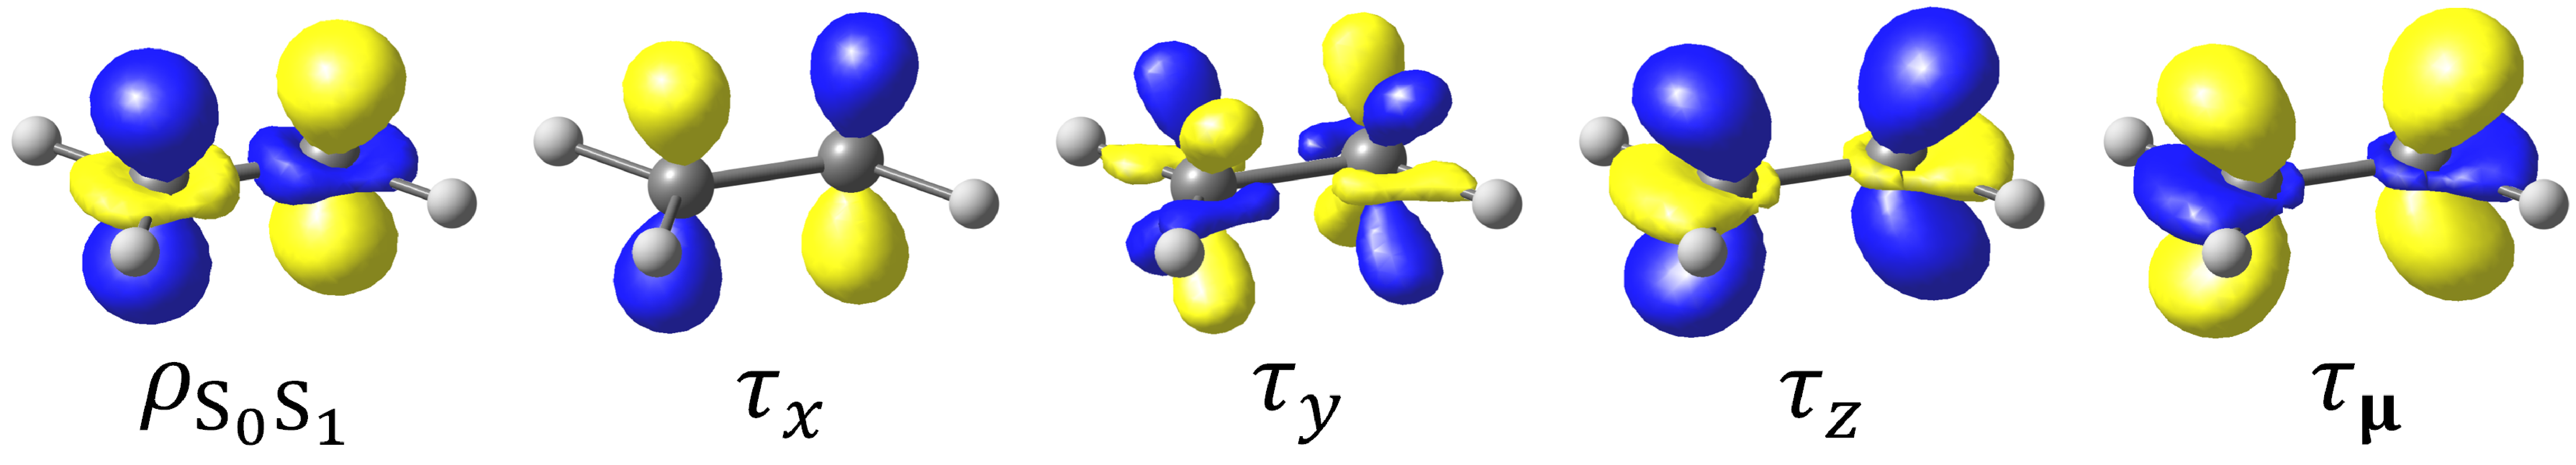
\includegraphics[width=15cm]{tdmd.eps}
\caption{
$\rho_{\mathrm{S}_0\mathrm{S}_1}$, $\tau_x$, $\tau_y$, $\tau_z$, and $\tau_{\bm{\upmu}}$ distributions.
Yellow shows positive; blue shows negative.
}
\label{fig:tdmd}
\end{figure}

%%%%%%%%%%%%%%%%%%%%%%%%%%%%%%%%%%%%%%%%%%%%%%%%%%%%%%%%%%%%%%%%%%%%%%%%%%%%%%%%%%%%%%%%%%%%
%%%%%%%%%%%%%%%%%%%%%%%%%%%%%%%%%%%%%%%%%%%%%%%%%%%%%%%%%%%%%%%%%%%%%%%%%%%%%%%%%%%%%%%%%%%%
\clearpage
\subsection{Vibronic coupling densities between S$_0$ and S$_1$ at optimized S$_0$ geometry}
This example shows how vibronic coupling densities are calculated with d77. 
Sample d77 input and output files are in the examples/C2H4/VCD directories. The first three steps are the same as in \bf{\ref{calc_VCC}}\rm{.}
\begin{enumerate}

\item{Run geometry optimization and frequency analysis with Gaussian 16. 6D and 10F options are required to run d77.}
\item{Generate freq.fchk and TD.fchk files.}
\item{Run dpp.}

\item{
Calculate vibronic coupling densities between S$_0$ and S$_1$.\\
Create VCD directory and move into it:
\begin{verbatim}
mkdir VCD
cd VCD
\end{verbatim} 
A sample input file (VCD\_0\_3.inp) is as follows:
\begin{verbatim}
$comment
Input file for calculating vibronic coupling densities
for S0-S1 transition
| 0 > : ground state (S0)
| 3 > : lowest excited singlet state (S1)
$end_comment

$control
property = vc
runtyp   = density
method   = td
$end_control

$elec_state
bra = < 0 |
ket = | 3 >
$end_elec_state

$vibmode
7
9
$end_vibmode

$grid
xmin = -5.0
xmax =  5.0
ymin = -5.0
ymax =  5.0
zmin = -5.0
zmax =  5.0
dx = 0.10
dy = 0.10
dz = 0.10
$end_grid

DIR_INP_ELEC  = ../INP_ELEC
DIR_INP_VIB   = ../INP_VIB
DIR_INP_ELFLD = ../ELFLD
\end{verbatim}
To run d77, type:
\begin{verbatim} 
d77 VCD_0_3 
\end{verbatim}
d77 calculates the S$_0$-S$_1$ overlap density ($\rho_{\mathrm{S}_0\mathrm{S}_1}$), 
the derivatives of the nuclear electronic potentials for the seventh and ninth vibrational modes ($\nu_7$ and $\nu_9$),
and the vibronic coupling densities for the seventh and ninth vibrational modes ($\eta_7$ and $\eta_9$).
The calculated $\rho_{\mathrm{S}_0\mathrm{S}_1}$, $\nu_7$, $\nu_9$, $\eta_7$, and $\eta_9$
are written to RHO.cube, DVNE0007.cube, DVNE0009.cube, VCD0007.cube, and VCD0009.cube files 
in the VCD\_0\_3 directory.
RHO.cube ($\rho_{\mathrm{S}_0\mathrm{S}_1}$) calculated in this example
is the same as that calculated in \bf{\ref{calc_RHO}}\rm{.}
You can skip generating RHO.cube by adding the following option in your control section:
\begin{verbatim} 
save_rho_cube = no
\end{verbatim}
}
\end{enumerate}

\indent
Figure \ref{fig:vcd} shows the $\rho_{\mathrm{S}_0\mathrm{S}_1}$, $\nu_7$, $\nu_9$, $\eta_7$, and $\eta_9$ distributions visualized with Chemcraft. $\nu_7$ and $\nu_9$ dsitributions reflect the seventh and ninth vibrational modes, respectively. $\eta_7$ and $\eta_9$ are calculated from the relations: $\eta_7 = \rho_{\mathrm{S}_0\mathrm{S}_1} \times \nu_7$; $\eta_9 = \rho_{\mathrm{S}_0\mathrm{S}_1} \times \nu_9$. The spatial integral of $\eta_7$ and $\eta_9$ gives VCCs for the seventh and ninth vibrational modes, respectively.

The $\eta_7$ distribution suggests that the vibronic coupling for the seventh vibrational mode occurs around the carbon atoms. 
The $\eta_9$ distribution suggests that the vibronic coupling for the ninth vibrational mode occurs along the C$-$H bonds.

\begin{figure}[h]
\centering
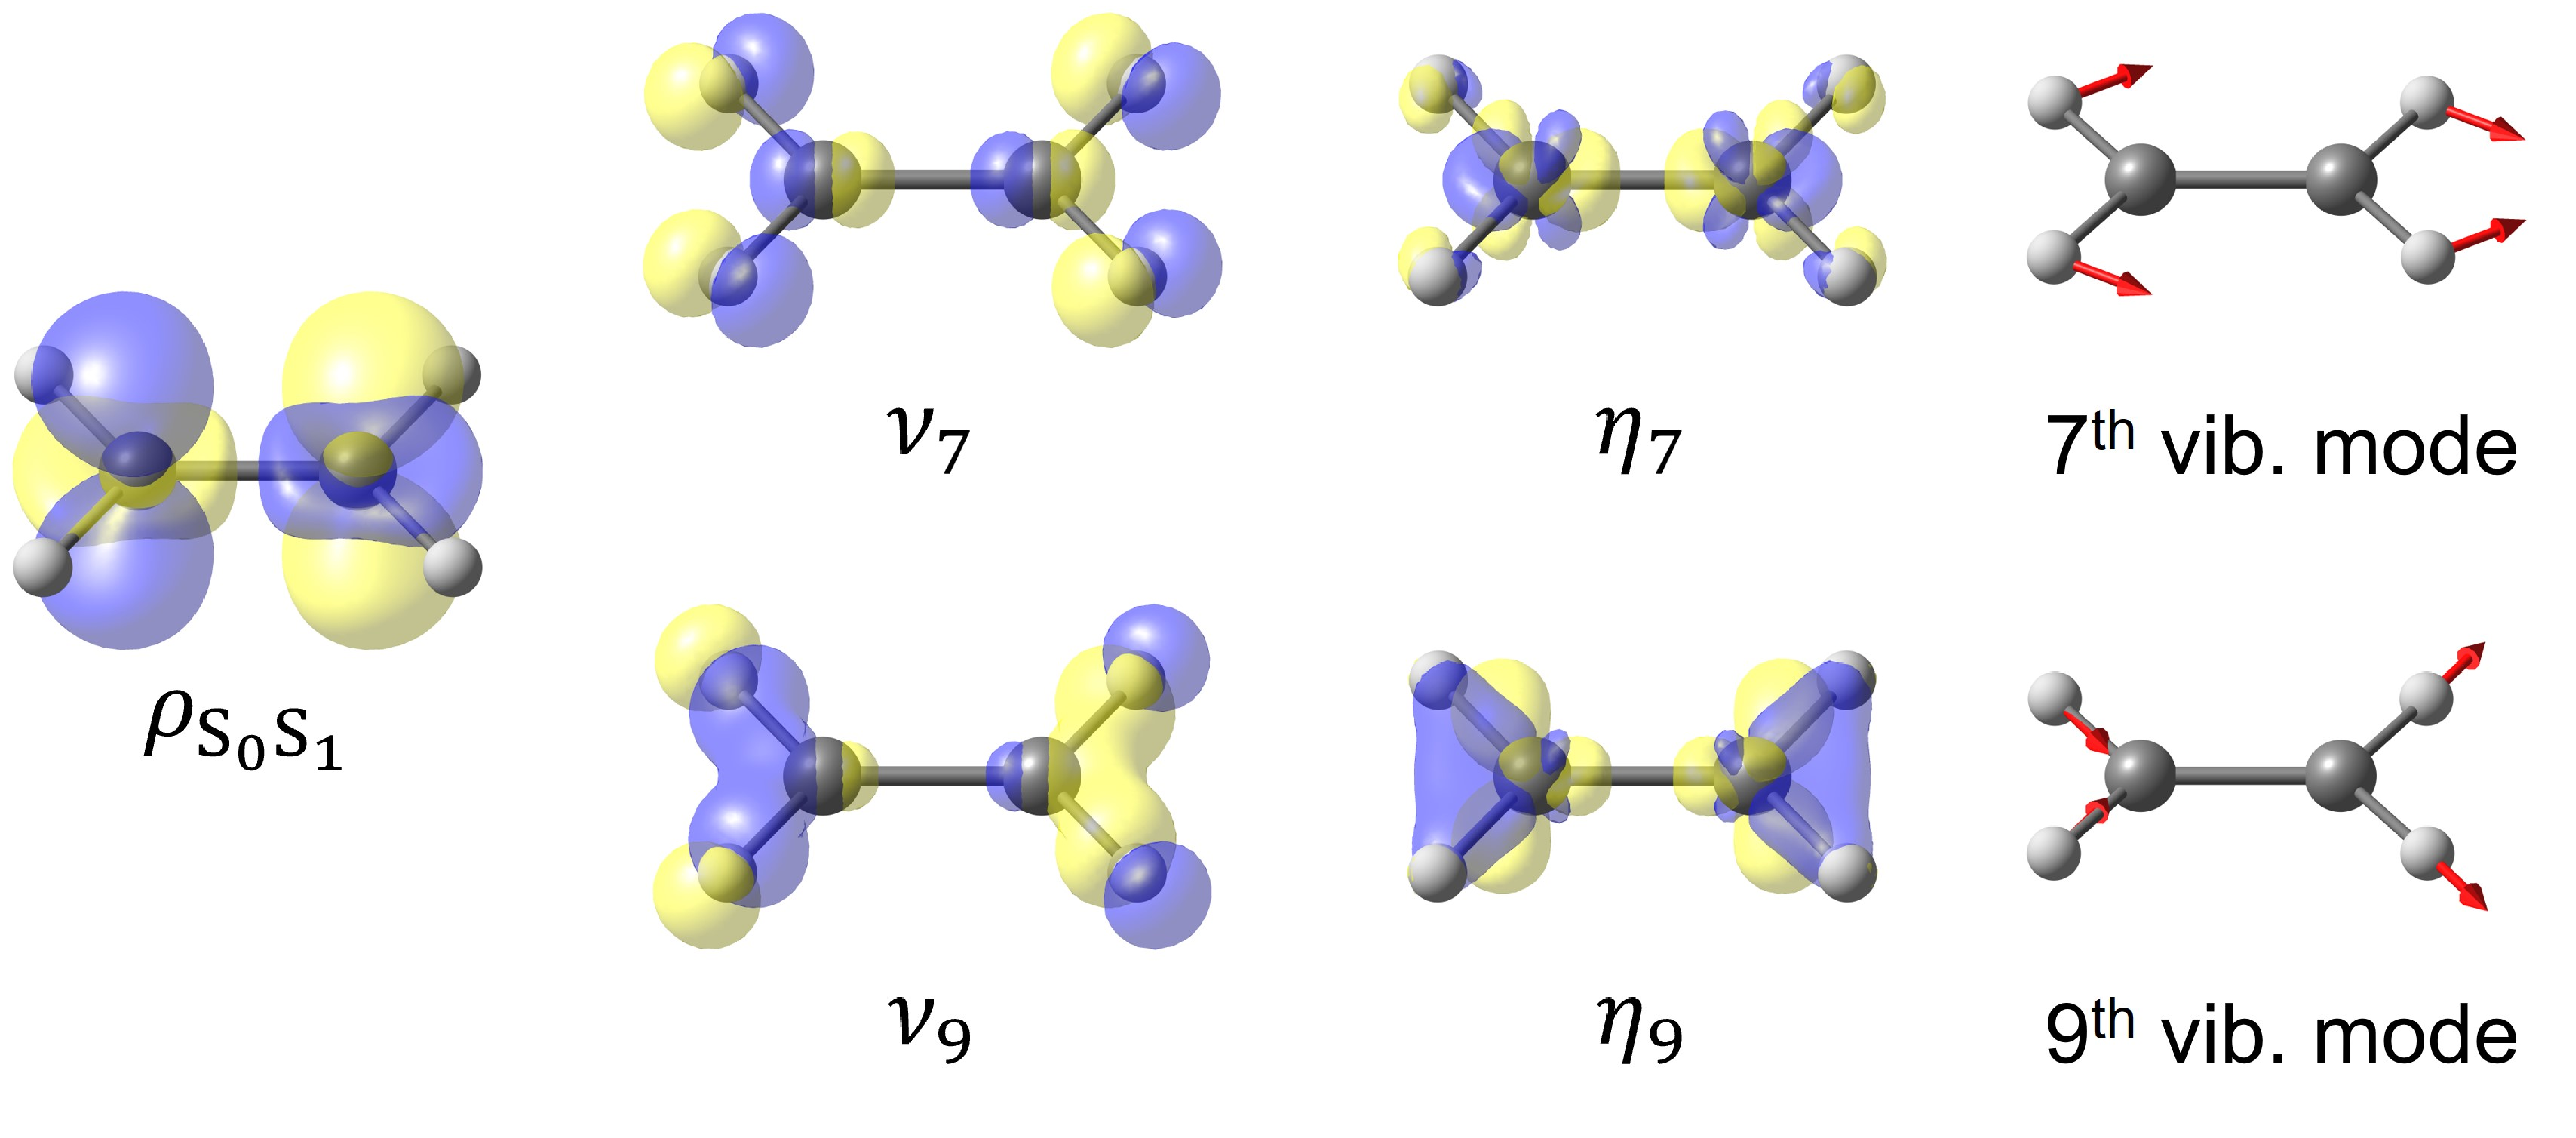
\includegraphics[width=15cm]{vcd.eps}
\caption{
$\rho_{\mathrm{S}_0\mathrm{S}_1}$, $\nu_7$, $\nu_9$, $\eta_7$, and $\eta_9$ distributions.
Yellow shows positive; blue shows negative.
}
\label{fig:vcd}
\end{figure}


%%%%%%%%%%%%%%%%%%%%%%%%%%%%%%%%%%%%%%%%%%%%%%%%%%%%%%%%%%%%%%%%%%%%%%%%%%%%%%%%%%%%%%%%%%%%
%%%%%%%%%%%%%%%%%%%%%%%%%%%%%%%%%%%%%%%%%%%%%%%%%%%%%%%%%%%%%%%%%%%%%%%%%%%%%%%%%%%%%%%%%%%%
\clearpage
\bibliographystyle{prsty}
\bibliography{d77.bib}
\end{document}
%%%%%%%%%%


